%% =====================================================================
%%  Emmanuel Kumah — Dribbble-inspired CV
%%  Compile with XeLaTeX or LuaLaTeX (Overleaf default works perfectly).
%%  Two-column sidebar layout, soft pastel palette, big bold name block.
%% =====================================================================
\documentclass[10pt,a4paper]{article}

\usepackage[a4paper, margin=0pt]{geometry}
\usepackage{fontspec}
\usepackage{xcolor}
\usepackage{tikz}
\usepackage{tcolorbox}
\usepackage{fontawesome5}
\usepackage{enumitem}
\usepackage{hyperref}
\usepackage{ragged2e}
\usepackage{anyfontsize}

\tcbuselibrary{skins,breakable}

% Try to use a friendly geometric sans — fall back gracefully.
\IfFontExistsTF{Fira Sans}{\setmainfont{Fira Sans}}{}
\newfontfamily\displayfont{Playfair Display}[
  UprightFont = * Regular,
  BoldFont    = * Bold,
  ItalicFont  = * Italic
]
\newfontfamily\monofont{JetBrains Mono}[Scale=0.85]

% --- Palette (matches portfolio site) ---------------------------------
\definecolor{ink}{HTML}{0D0D18}
\definecolor{inkSoft}{HTML}{303046}
\definecolor{inkMute}{HTML}{6B6B85}
\definecolor{cream}{HTML}{FDFCF9}
\definecolor{creamDeep}{HTML}{F3EFE6}
\definecolor{accent}{HTML}{E63995}
\definecolor{accentDeep}{HTML}{A01060}
\definecolor{electric}{HTML}{5B62E4}
\definecolor{cyanGlow}{HTML}{0BB5D4}
\definecolor{mint}{HTML}{14B88A}
\definecolor{amber}{HTML}{F59E0B}

\hypersetup{
  colorlinks=true,
  urlcolor=accentDeep,
  pdftitle={Emmanuel Kumah — CV},
  pdfauthor={Emmanuel Kumah}
}

\pagestyle{empty}
\setlist[itemize]{leftmargin=*, label={\textcolor{accent}{\small\faCircle[regular]}}, itemsep=2pt, topsep=2pt}

% --- Reusable bits ----------------------------------------------------
\newcommand{\sectiontitle}[2]{%
  {\displayfont\bfseries\fontsize{14}{16}\selectfont\color{ink} #1}\hspace{0.4em}%
  {\color{accent}\rule[0.25ex]{1.6cm}{1.2pt}}\par
  \ifx&#2&\else\vspace{-2pt}\textcolor{inkMute}{\small #2}\par\fi
  \vspace{6pt}
}

\newcommand{\sidesection}[1]{%
  \vspace{10pt}%
  {\displayfont\bfseries\fontsize{12}{14}\selectfont\color{white} #1}\par
  {\color{accent}\rule{2.2cm}{1.2pt}}\par
  \vspace{4pt}
}

% Experience entry: role, company, period, location, blurb, bullets
\newcommand{\role}[5]{%
  \vspace{4pt}
  \noindent\begin{minipage}{\linewidth}
    {\bfseries\color{ink}\fontsize{11.5}{13}\selectfont #1}\hfill
    {\color{accent}\monofont\footnotesize #4}\par
    {\color{electric}\bfseries #2}\hspace{0.4em}{\color{inkMute}\footnotesize · #3}\par
    \vspace{2pt}
    {\color{inkSoft}\small\justifying #5}\par
  \end{minipage}\\[2pt]
}

% Project entry: title, stack, blurb
\newcommand{\projectcard}[3]{%
  \begin{tcolorbox}[
    enhanced, breakable,
    colback=creamDeep!50, colframe=accent!25,
    boxrule=0.6pt, arc=4pt, left=10pt, right=10pt, top=8pt, bottom=8pt,
    width=\linewidth
  ]
    {\bfseries\color{ink}\fontsize{10.5}{12}\selectfont #1}\par
    {\monofont\scriptsize\color{electric} #2}\par
    \vspace{3pt}
    {\color{inkSoft}\footnotesize\justifying #3}
  \end{tcolorbox}
  \vspace{2pt}
}

% Skill chip
\newcommand{\chip}[1]{%
  \tikz[baseline=(c.base)]\node[
    fill=white, draw=accent!40, line width=0.4pt,
    rounded corners=3pt, inner xsep=5pt, inner ysep=2pt,
    text=ink, font=\monofont\scriptsize
  ] (c) {#1};%
}

% =====================================================================
\begin{document}
\sffamily

% Page background = soft cream
\begin{tikzpicture}[remember picture, overlay]
  \fill[cream] (current page.south west) rectangle (current page.north east);

  % Decorative dot grid in top-right
  \foreach \x in {0,1,...,8}{
    \foreach \y in {0,1,...,5}{
      \fill[ink!10] ([xshift=-2.2cm-\x*0.32cm, yshift=-0.8cm-\y*0.32cm] current page.north east)
        circle (0.04cm);
    }
  }

  % --- Sidebar (left, ~6.2cm) ---------------------------------------
  \fill[ink] (current page.south west) rectangle
    ([xshift=6.2cm] current page.north west);

  % Pink accent strip behind sidebar header
  \fill[accent] ([xshift=0cm, yshift=-3.6cm] current page.north west) rectangle
    ([xshift=6.2cm, yshift=-4cm] current page.north west);
\end{tikzpicture}

% =====================================================================
%  CONTENT
% =====================================================================
\noindent
\begin{minipage}[t]{6.2cm}\color{white}
  \vspace{1.2cm}
  \begin{center}
    % Photo in a circular frame
    \begin{tikzpicture}
      \clip (0,0) circle (2.1cm);
      \node[inner sep=0pt] at (0,0)
        {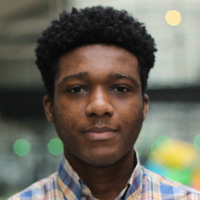
\includegraphics[width=4.6cm]{photo.jpg}};
      \draw[white, line width=2pt] (0,0) circle (2.1cm);
    \end{tikzpicture}
  \end{center}

  \vspace{0.4cm}
  \begin{center}
    {\monofont\small\color{accent}FULL\,-\,STACK ENGINEER}
  \end{center}

  \vspace{0.8cm}
  \hspace{0.6cm}\begin{minipage}{5.0cm}\RaggedRight

  \sidesection{Contact}
  \small
  \faEnvelope[regular]\ \href{mailto:emmanuel.kumah.dev@gmail.com}{\color{white}emmanuel.kumah.dev}\\
  \faGlobe\ \href{https://easyblend.me}{\color{white}easyblend.me}\\
  \faGithub\ \href{https://github.com/easyblend}{\color{white}easyblend}\\
  \faLinkedin\ \href{https://www.linkedin.com/in/emmanuel-kumah-692431224/}{\color{white}emmanuel-kumah}\\
  \faTwitter\ \href{https://twitter.com/bug_inspector}{\color{white}bug\_inspector}\\
  \faMapMarker*\ \textcolor{white!80}{Paris, France}

  \sidesection{Toolbox}
  \begin{flushleft}
    {\color{accent}\textbf{Front-end}}\\
    \footnotesize\color{white!90}React · TypeScript · Next.js · Tailwind · Framer\par
    \vspace{4pt}
    {\color{accent}\textbf{Back-end}}\\
    \footnotesize\color{white!90}Java · Spring Boot · Python · FastAPI · Node\par
    \vspace{4pt}
    {\color{accent}\textbf{Data \& Cloud}}\\
    \footnotesize\color{white!90}PostgreSQL · Supabase · Docker · GitHub Actions · Jenkins · Vercel\par
    \vspace{4pt}
    {\color{accent}\textbf{Testing \& Perf}}\\
    \footnotesize\color{white!90}Jest · RTL · K6 · OctoPerf · Playwright\par
  \end{flushleft}

  \sidesection{Languages}
  \footnotesize
  \color{white!90}
  English {\color{accent}\faCircle\faCircle\faCircle\faCircle\faCircle}\par
  French \hspace{0.45em} {\color{accent}\faCircle\faCircle\faCircle\faCircle}\faCircle[regular]\par
  Akan \hspace{0.85em} {\color{accent}\faCircle\faCircle\faCircle\faCircle\faCircle}\par

  \sidesection{Education}
  \footnotesize\color{white!90}
  \textbf{M.Sc. Computer Science}\\
  IT University · Paris\\
  {\color{white!60}\monofont\scriptsize 2023 — 2025}\par
  \vspace{6pt}
  \textbf{B.Sc. Computer Science}\\
  KNUST · Kumasi, Ghana\\
  {\color{white!60}\monofont\scriptsize 2018 — 2022}

  \sidesection{Highlights}
  \footnotesize\color{white!90}
  {\color{accent}\faTrophy}\ \ 90\% test coverage on critical flows\\[2pt]
  {\color{accent}\faRocket}\ \ 40\% drop in manual QA effort\\[2pt]
  {\color{accent}\faBolt}\ \ 15\% page-load improvement\\[2pt]
  {\color{accent}\faUsers}\ \ Aligned 20+ engineers across 5 countries

  \end{minipage}
\end{minipage}\hfill
% ---------------------------------------------------------------------
\begin{minipage}[t]{\dimexpr\textwidth-6.2cm-1.2cm\relax}
  \vspace{1.2cm}\hspace{0.4cm}\begin{minipage}{\linewidth-0.4cm}

  % --- Hero name block --------------------------------------------
  \noindent
  {\monofont\small\color{accent}\textbf{HELLO, I'M}}\par
  \vspace{2pt}
  {\displayfont\bfseries\fontsize{34}{38}\selectfont\color{ink}Emmanuel}\par
  {\displayfont\bfseries\fontsize{34}{38}\selectfont\color{accent}Kumah.}\par
  \vspace{6pt}
  {\color{inkSoft}\fontsize{11}{14}\selectfont
    Full-stack engineer crafting elegant interfaces and
    rock-solid backends — from climate-tech dashboards
    at Station F to AI fraud-detection at Shift Technology.}
  \par
  \vspace{14pt}
  {\color{accent}\rule{2.2cm}{1.4pt}}\hspace{4pt}%
  {\color{electric}\rule{1.4cm}{1.4pt}}\hspace{4pt}%
  {\color{cyanGlow}\rule{0.7cm}{1.4pt}}
  \vspace{14pt}

  % --- PROFILE ----------------------------------------------------
  \sectiontitle{Profile}{}
  {\color{inkSoft}\small\justifying
  I build products end-to-end — pixel-perfect React frontends,
  type-safe APIs, and the CI/CD pipelines that ship them. I love
  obsessing over DX, performance budgets, and the tiny details that
  make software feel good to use.}
  \vspace{10pt}

  % --- EXPERIENCE -------------------------------------------------
  \sectiontitle{Experience}{}

  \role{Software Engineer — Quality \& Platform}
    {Shift Technology}
    {Paris, France}
    {Mar 2025 — Now}
    {Force is Shift's AI fraud-detection SaaS for tier-1 insurers
     (AXA, Allstate \& others, 10K+ MAU). Led a multi-month POC
     comparing K6 (CLI + Browser) vs OctoPerf for UI perf testing
     across React, Java, C\# and Python services — selected
     \textbf{OctoPerf} as Shift's official tool and aligned 20+ engineers
     across 5 countries. Designed the AXA FR test plan (10\,$\to$\,40 VUs,
     15-min loads, P95/P99 + Grafana CPU/RAM on Azure PWS1 / PDB3 / PCP3);
     uncovered a doc-upload saturation point at 40 VUs (CPU $\sim$89\%,
     2.1\% error rate) and search-endpoint timeouts past 12 min.
     Shipped 20+ reusable K6 + OctoPerf scenarios in CI (Jenkins,
     GitHub Actions, Docker) — \textbf{-40\% manual QA effort,
     +30\% regression coverage}. Authored the team OctoPerf playbook
     (HAR/Firefox correlation, regex extractors, on-prem Docker,
     no-internet Azure VM via scp + SSH port-forwarding). Now in the
     Services Squad driving QA for SCIM US rollout (Allstate),
     Document Storage in Japan (JPE1), Allstate external-worker
     service, and a doc-service 404 flakiness investigation.
     Hardened critical Force UI paths to 90\% test coverage and
     drove a 15\% page-load improvement.}

  \role{Frontend Engineer — Intern \& Freelance}
    {STATION F · Kanop}
    {Paris, France}
    {Mar 2024 — Feb 2025}
    {Owned frontend delivery for a climate-tech web platform.
     Built a type-safe React + TypeScript UI on top of new REST APIs
     via React Query; introduced Jest \& RTL and reached 90\% coverage
     on critical flows; shipped UX upgrades that moved product KPIs.}

  \role{Founder \& Engineer}
    {CrowdTest.dev}
    {Side project · 2025 — Now}
    {Live SaaS (\href{https://crowdtest.dev}{crowdtest.dev}) connecting
     devs with real human testers for pre-launch bug-hunting.
     Next.js 16 monorepo (marketing + product) on Prisma 7 + Postgres;
     3-role RBAC on Supabase Auth enforced via edge middleware + HTTP-only
     JWT cookies; full bug pipeline (React Hook Form $\to$ Cloudinary upload
     $\to$ Prisma transaction $\to$ audit log $\to$ owner email);
     append-only audit log surfaced in an admin dashboard; secret-gated
     weekly Vercel Cron digest emails via Brevo SMTP.}

  \vspace{6pt}

  % --- PROJECTS ---------------------------------------------------
  \sectiontitle{Selected Projects}{}

  \projectcard{CrowdTest.dev — Crowd Testing SaaS}
    {Next.js 16 · Prisma · Postgres · Supabase · Cloudinary · Brevo · Vercel}
    {Live SaaS pairing devs with real human testers; RBAC, audit log,
     Cloudinary screenshots and weekly Vercel-Cron email digests.}

  \projectcard{Spatial Showdown — Multiplayer Game}
    {React · Three.js · Socket.IO · Node}
    {Real-time online multiplayer 3D arena with WebSocket-driven
     matchmaking and physics-synced gameplay.}

  \projectcard{Flexicoins — Web3 Wallet}
    {React · Solidity · Ethers · Hardhat}
    {Lightweight EVM wallet with portfolio analytics, multi-chain
     support, and signed-transaction flows.}

  \projectcard{BioSample — LIMS Web App}
    {React · Spring Boot · PostgreSQL · Docker}
    {Lab sample management system used by research teams to track
     biological samples, chains of custody and analyses.}

  \end{minipage}
  \vspace{1.2cm}
\end{minipage}

\end{document}
